\chapter{The nEDM apparatus}
\label{ch:nedm-at-psi-apparatus}

As in the UKy presentation:

First about the history of the experiment, the collaboration, when was it taking data, that it was disassembled in Autumn 2017. Has enough statistics to set the world's best limit. The analysis still ongoing.

Thou shall measure frequency
What frequency? - Measurement principle.
The neutron is a spin-one-half particle. In a magnetic field the hamiltonian is.
Then in 
\note{need to check that carefully}
So we measure a change in the spin-up--spin-down transition frequency between the magnetic and electric field being parallel and anti-parallel.

\begin{figure}
  \centering
  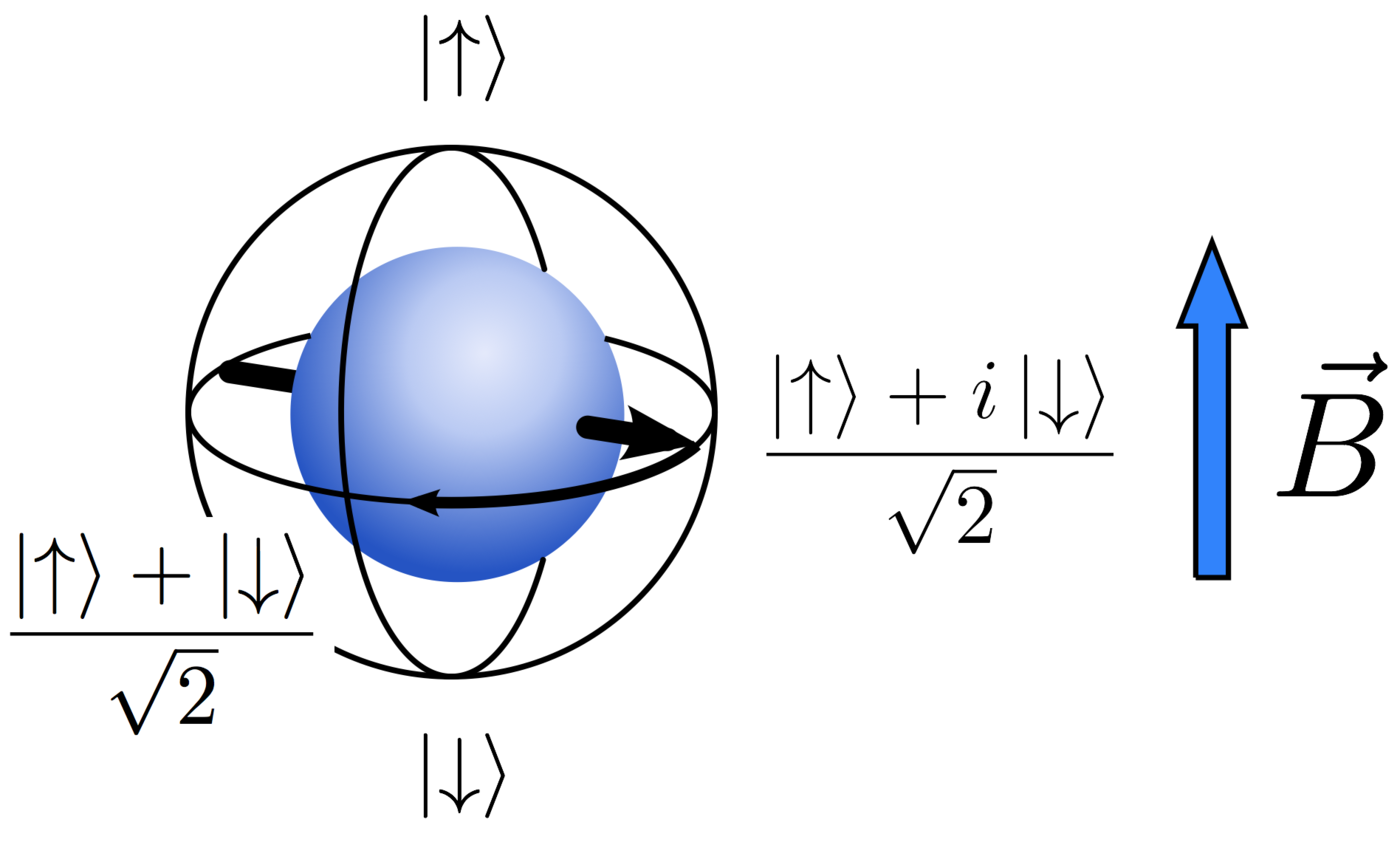
\includegraphics[width=.6\linewidth]{gfx/nEDMatPSI/bloch_sphere.png}
  \caption{\ldots}
  \label{fig:nEDM_bloch_sphere}
\end{figure}

How is this frequency measured? Larmor precession, then Ramsey method.
Then the Bloch sphere, a nice picture of the spin.
Then the ramsey measurement principle.

\begin{SCfigure}
  \centering
  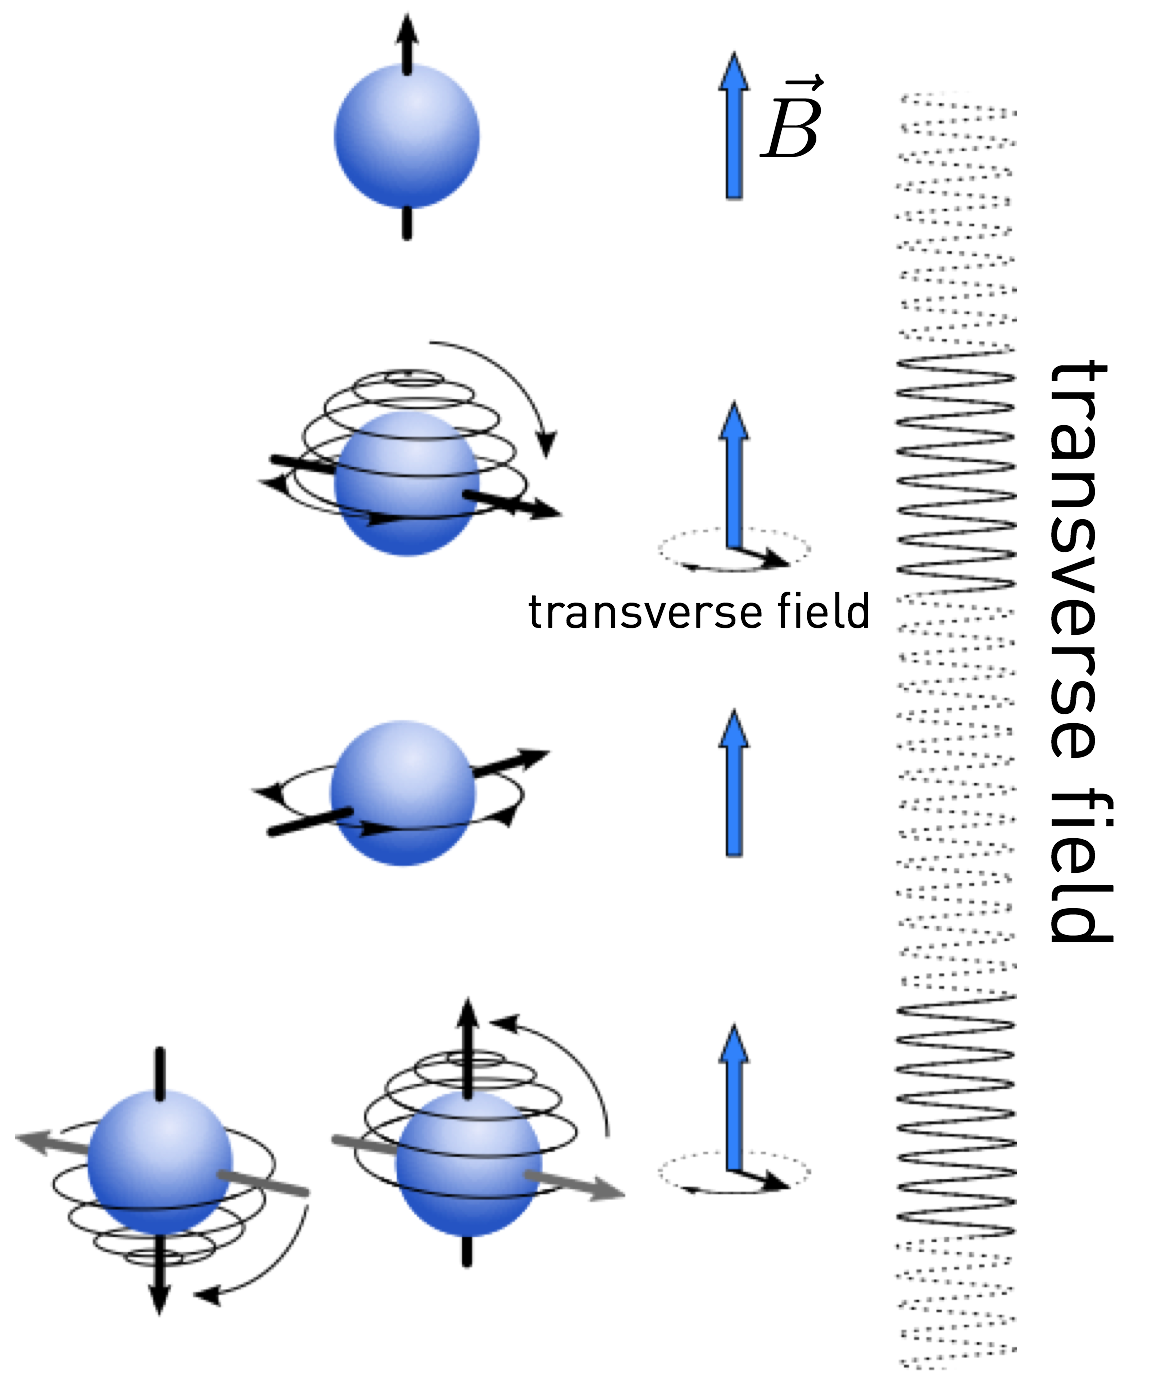
\includegraphics[width=.6\linewidth]{gfx/nEDMatPSI/Ramsey_principle.png}
  \caption{\ldots}
  \label{fig:nEDM_Ramsey_principle}
\end{SCfigure}


How is it realised in practice?
UNCs, curcial.
The the apparatus, still in the context of the Ramsey measurement.
Already with the procedure, somehow.

Finally, the importance of the magnetic field.













Description of the experimental setup and the measurement procedure.

\subsection{The Sussex-RAL-ILL Room Temperature Neutron Electric Dipole Moment Experiment}
\note{NA: this subsection is still a very early draft, I know there are still formatting issues and blanks}

\note{This first bit is paraphrased from C.A. Baker et al., Apparatus for Measurement of the Electric Dipole Moment of the Neutron using a Cohabiting Atomic-Mercury Magnetometer}

\note{MR: This should probably be made much shorter.}

Most experiments to measure the static electric dipole moment of the neutron use magnetic resonance techniques to observe the Larmor precession of free neutrons in parallel and antiparallel magnetic and electric fields. The Hamiltonian of an uncharged spin $1/2$ particle in an electric and a magnetic field is:
\begin{equation}
H = - 2\vec{S} \cdot (\mu \vec{B} + d \vec{E})
\end{equation}
In the case of parallel and antiparallel magnetic and electric fields, this gives a precession frequency of:
\begin{equation}
h\nu = -2\mu B \mp 2dE
\end{equation}
In the presence of a non-zero EDM, when the direction of the applied electric field is reversed relative to the magnetic field we expect a shift in the precession frequency of
\begin{equation}
\delta \nu _0 = −\frac{4d_n E_0}{h} .
\end{equation}
In the Sussex-RAL-ILL Room Temperature experiment, polarised ultracold neutrons produced at the fundamental physics beamline at the ILL high flux reactor were stored in a material bottle (a cylinder of diameter 235mm and height 120mm), wherein their precession frequency in parallel and antiparallel combinations of electric and magnetic fields was measured using the Ramsey Technique. To combat drifts in the magnitude of the applied magnetic field, a cohabiting magnetometer of atomic $^{199}$Hg was used, and analysis was done by considering the ratio of neutron and mercury precession frequencies, “$R$”.

Each measurement sequence (“cycle”) consisted of a filling period, a first $\pi/2$ pulse to rotate the neutron spins into the horizontal plane, a 130s period of free precession, a second $\pi/2$ pulse to project the spins onto the z axis, and an emptying period where the number of spin-up and spin-down neutrons were counted. The precession of the mercury during the free precession period was measured by observing the modulation of the absorption of light from a mercury discharge lamp \note{is it actually a discharge lamp?}. Each cycle lasted in total x minutes. Many cycles were taken at each fixed magnetic field configuration over the course of between 1 and 73 hours (a “run”), while the direction of the applied electric field was reversed every 20 cycles. From each run a value of the neutron to mercury frequency ratio $R$ was extracted, as well as a value of the apparent EDM.

As a result of a conspiracy between radial magnetic field components and rotating magnetic components arising from the Lorentz transformation of the large applied electric field into the rest frame of the mercury atoms, a frequency shift proportional to the applied electric field was observed, mimicking the effect of a non-zero electric dipole moment of the neutron --- a “false EDM”. This effect is, however, directly proportional to the gradient of the applied vertical magnetic field dBz/dz, and reverses with the sign of the applied magnetic field. The false EDM effect has been analysed in more detail in \note{cite false edm paper(s)} and a direct measurement of this effect was made in \note{cite false edm measurement}.

As the ILL experiment had no direct measurement of the vertical gradient, the measurement of the neutron to mercury frequency ratio was instead used as a proxy. Due to the extremely low energy of the ultracold neutron population, the centre of mass of the neutron population sags a little below the centre of the precession chamber. The relatively hot population of mercury atoms does not suffer from this effect, so there is an effective height difference $\Delta h \approx 3.7 \mathrm{mm}$ between the neutron and mercury populations. Thus, the ratio of neutron to mercury frequencies depends (to first order) on the vertical gradient like: \note{MR: We might want to get rid of the stacked fraction for clarity.}
\begin{equation}
  R = R_0 \left( 1 + \Delta h  \frac{\frac{\mathrm{d}B_z}{\mathrm{d}z}}{B_{0}} \right).
  \label{eq:R}
\end{equation}
This frequency shift does not uniformly affect the entire neutron population: the effect is much greater for the lowest energy neutrons which have a lower centre of mass. This causes a departure from the linear relation above; however, in the low vertical gradient regime ($\lesssim 30 \mathrm{pT/cm}$) in which most of the data was taken, the effect is almost exactly linear. This effect is described more thoroughly in [cite grav depol papers].

To correct for these false EDMs in static EDM searches, the “crossing lines” procedure was adopted.  For each direction of the magnetic field, the measured EDM value was plotted against the measured neutron to mercury frequency ratio. Barring other systematic shifts, it is considered that the vertical gradient is zero where these lines cross. Other effects arising from transverse magnetic fields, the rotation of the earth and cause additional frequency shifts in the neutrons or in the cohabiting magnetometer, which can \note{PH: no it isn't -- there are still systematics from e.g. transverse fields, which can move the crossing point away from dB/dz=0, in addition to effects such as Earth's rotation that result in a vertical shift of the crossing point...]}, and therefore a measurement of the neutron electric dipole moment independent of the false EDM effect and of the neutron to mercury frequency ratio independent of the gravitational shift can be extracted. In the rest of the run-level analysis, we work with data where these false EDM effects have been subtracted. Further systematic effects shift the measured neutron to mercury frequency ratio or the measured EDM value, however these effects can be assumed to have been constant throughout the entire experimental measurement period, and so will not be further explored in this analysis. Systematic effects affecting the static analysis of the ILL experiment are explored in depth in [cite reanalysis] and [cite apparatus paper].

\note{MR: Need to mention explicitly, that the average $d_n$ over a run is measured (though not exactly, it is only over the free precession periods), and this is how it is treated in the Monte Carlo simulations.}


\section{nEDM @ PSI data taking scheme}
The nEDM experiment at PSI probes the Ramsey resonance curve of ultra--cold neutrons (\emph{UCNs}). Its operation consists of subsequent \emph{cycles}, wherein an ensemble of polarised \emph{UCNs} undergoes a Ramsey cycle in a magnetic field. At the end the polarisation of the ensemble is measured. The measurement is performed in a controllable electric field, which takes up three values: parallel to the magnetic field, antiparallel to it and zero. The electric field configuration is altered every couple of tens of cycles.

The Ramsey resonance curve of the neutrons is probed only in four \emph{working points}, as shown in Fig.\,\ref{fig:axions_working_points}. The points lie on the curve's steep slope. Thereby the resonance position is determined more precisely then it would should the curve be probed homogeneously or close to the resonance.

\begin{figure}[bth]
  \myfloatalign
  \subfloat
  [The \emph{working points} method. The plot depicts the measured neutron polarisation in function of the $pi/2$ pulses frequency. The frequencies are normalised by appropriate gyromagnetic ratios.]
  {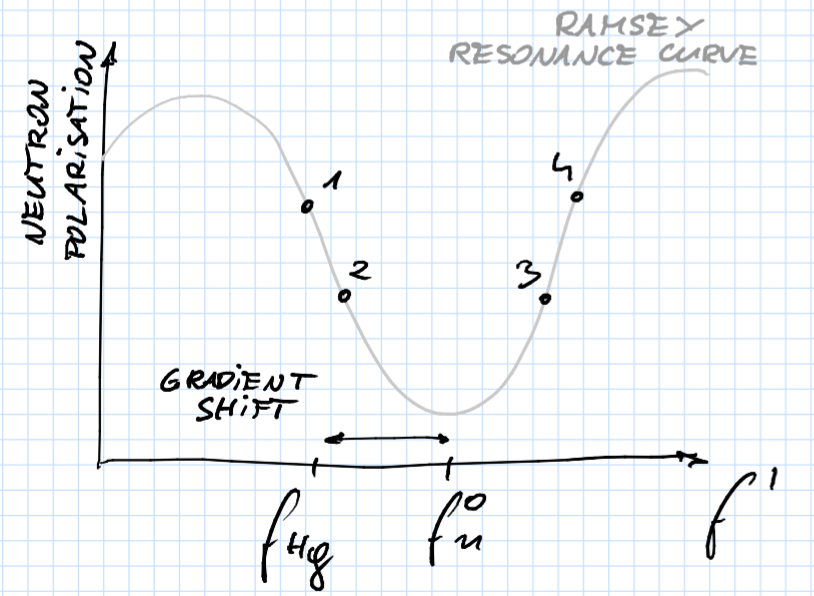
\includegraphics[width=.45\linewidth]{gfx/axions/data_taking_working_points}}
  \quad
  \subfloat
  [The \emph{working points} are probed subsequently.]
  {\label{fig:example-b}
  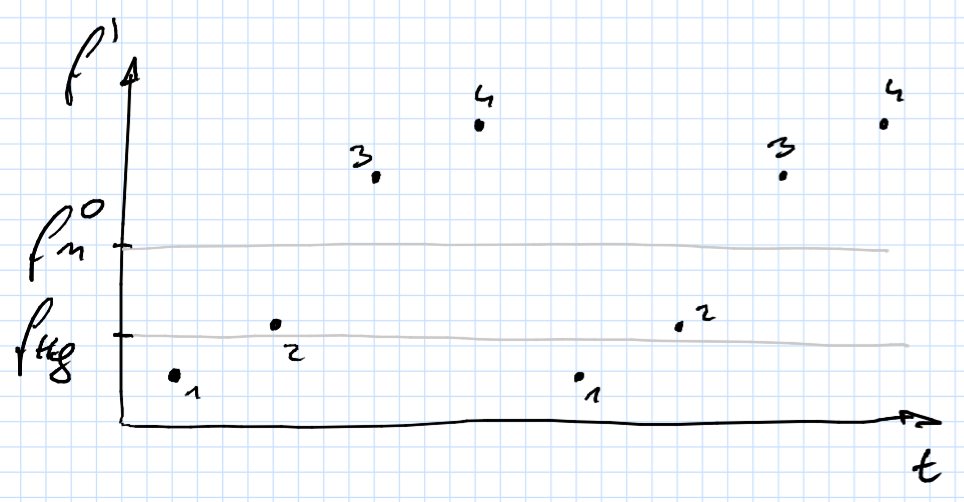
\includegraphics[width=.45\linewidth]{gfx/axions/data_taking_working_points_time}}
  \caption{The principle of working points}
  \label{fig:axions_working_points}
\end{figure}

The resonance frequency $f_n^{\,0}$ is determined with a fit of the resonance curve. Because the points are probed one after another, it is only possible after a set of data points, \emph{cycles}, have been measured. In order to extract the neutron precession frequency for each individual \emph{cycle}, one assumes that the only parameter of the resonance curve that varies on a cycle--to--cycle basis is the position of the resonance. With this assumption the shape of the curve, fitted to the whole set of \emph{cycles}, is used to calculate back the resonant frequency in each \emph{cycle} of the set.

Together with the UCNs there is a polarised $^{199}$Hg gas precessing. Its precession is monitored with light, allowing for direct determination of the $^{199}$Hg Larmor frequecy and thus the magnetic field strength. In order to cancel the first-order magnetic field changes one looks at the value:
\begin{equation}
  R := f_n / f_{Hg} \ .
\end{equation}
However, the UCNs are cold enough to have their centre of mass shifted downwards a few centimeters by the gravity. The $^{199}$Hg gas, being much hotter then the UCNs, fills the precession volume homogeneously. In a presence of a vertical magnetic field gradient this causes the two species to see different magnetic fields.

In the nEDM experiment at PSI data taking is divided into \emph{runs}. A single \emph{run} is carried out automatically with, in most cases, no human intervention. The machine cycles through the working points by itself. Also the charging of the electrodes creating the electric field is automatised. In between \emph{runs} manual interference happens, most importantly the magnetic field vertical gradient is altered.

In order to mitigate the bias due to the human factor, the nEDM experiment implements \emph{data blinding}. The data is artificially altered in a way that mimics a non--zero neutron electric dipole moment, big enough to be visible in the data. The exact value is secret and will be revealed only after the analysis is complete.
